\documentclass[nooutcomes]{ximera}
\input{../preamble}


\author{Bobby Ramsey}
\license{Creative Commons Attribution 4.0 International License}
%\acknowledgement{https://www.stitz-zeager.com/szca07042013.pdf}
\licenseSZ

\title{Applications of Trigonometry}

\begin{document}

\begin{abstract}
	
\end{abstract}
\maketitle


%\typeout{************************************************}
%\typeout{Review Questions}
%\typeout{************************************************}

%\section{Review Materials}
%    \begin{itemize}[label=\textbullet]
%	\item \link[Combining Like Terms]{https://spot.pcc.edu/math/orcca/ed2/html/section-combining-like-terms.html}
%	\item \link[Algebraic Properties and Simplifying Expressions]{https://spot.pcc.edu/math/orcca/ed2/html/section-algebraic-properties-and-simplifying-expressions.html}
%   \end{itemize}
%\begin{motivatingQuestions}\begin{itemize}
	%Often start a section. 
%	\item How can we define trigonometric functions for angles that do not come from triangles?
%\end{itemize}\end{motivatingQuestions}

\section{Applications of Trigonometry}

In the previous sections, you have been learning about trigonometric functions in the abstract. In this section, we wish to apply them.

\begin{example}

	A wire 200 meters long is attached to the top of a tower. When pulled taut, it makes a $60^\circ$ angle with the ground. How tall is the tower?
	How far away from the base of the tower does the wire hit the ground?
	
	\begin{explanation}
	
		In application problems, we are often given data about angles measured in degrees. It is up to us to translate this into radians for our 
		calculations. Let's call the angle we're given as $\theta$, so $\theta = \frac{\pi}{3}$ radians. Let's draw a diagram of this situation.

		\begin{image}[2in]
		  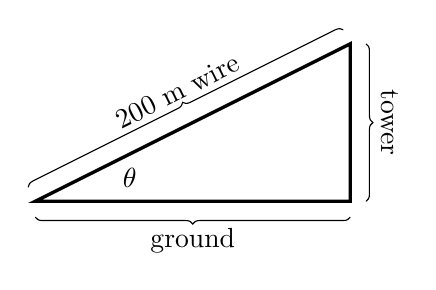
\begin{tikzpicture}
		    \coordinate (C) at (0,2);
		    \coordinate (D) at (4,2);
		    \coordinate (E) at (4,4);
		    \tkzMarkRightAngle(C,D,E)
		    \tkzMarkAngle(D,C,E)
		    \draw[decoration={brace,mirror,raise=.2cm},decorate,thin] (0,2)--(4,2);
		    \draw[decoration={brace,mirror,raise=.2cm},decorate,thin] (4,2)--(4,4);
		    \draw[decoration={brace,raise=.2cm},decorate,thin] (0,2)--(4,4);
		    \draw[very thick] (D)--(E)--(C)--cycle;
		    \node at (2,2-.5) {ground};
		    \node[rotate=-90] at (4+.5,3) {tower};
		    \node[rotate=26.5] at (2-.2,3+.4) {$200$ m wire};
		    \node at (1.2,2.3) {$\theta$};
		  \end{tikzpicture}
		\end{image}
		
		Based on this image, the height of the tower is the opposite the angle we know, and the distance along the ground is adjacent. That means
		the tower height is related to the angle by $\sin\left(\theta\right) = \frac{\text{tower}}{200}$ and the distance across the ground is given by
		$\cos\left(\theta\right) = \frac{\text{ground}}{200}$.
		
		Since $\sin\left( \frac{\pi}{3} \right) = \frac{\sqrt{3}}{2}$, the tower height can be computed by:
		\begin{align*}
			\sin\left(\frac{\pi}{3}\right) &= \frac{\text{tower}}{200}\\
			\text{tower} &= 200\sin\left(\frac{\pi}{3}\right)\\ 
				&= 200\left( \frac{\sqrt{3}}{2} \right)\\
				&= 100\sqrt{3}.
		\end{align*}
		The tower has a height of $100\sqrt{3}$ m, which is approximately $173.21$ m. 
		\begin{callout}
			The EXACT VALUE of the height is $100\sqrt{3}$ m. Saying that this is approximately $173.21$ m is provided to give us an indication of scale.
			Our actual answer is the exact value, not this approximation.
		\end{callout}
		We'll follow a similar calculation to find the distance from the base of the tower to the wire along the ground.
		\begin{align*}
			\cos\left(\frac{\pi}{3}\right) &= \frac{\text{ground}}{200}\\
			\text{ground} &= 200\cos\left(\frac{\pi}{3}\right)\\ 
				&= 200\left( \frac{1}{2} \right)\\
				&= 100.
		\end{align*}
		The wire hits the ground $100$ m from the base of the tower.
	\end{explanation}
\end{example}


\begin{example}
	
	A camera is setup 200 m from the base of a building, pointed at the top of the building. If the angle-of-elevation is measured as $76^\circ$, find the height of the building.
	
	\begin{explanation}
		
		The angle-of-elevation means the angle between the camera's line-of-sight and horizontal. Since the camera is setup 200 meters from the building, this gives us a right triangle where we know the
		base angle and the length of the adjacent side.
		
		If we call the height of the building as $h$, then we have a triangle
		\begin{image}[2in]
		  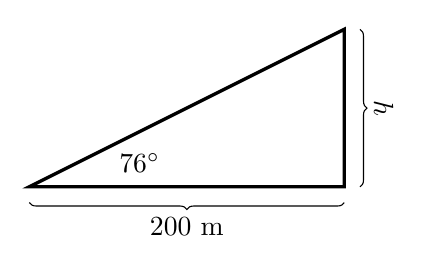
\begin{tikzpicture}
		    \coordinate (C) at (0,2);
		    \coordinate (D) at (4,2);
		    \coordinate (E) at (4,4);
		    \tkzMarkRightAngle(C,D,E)
		    \tkzMarkAngle(D,C,E)
		    \draw[decoration={brace,mirror,raise=.2cm},decorate,thin] (0,2)--(4,2);
		    \draw[decoration={brace,mirror,raise=.2cm},decorate,thin] (4,2)--(4,4);
%		    \draw[decoration={brace,raise=.2cm},decorate,thin] (0,2)--(4,4);
		    \draw[very thick] (D)--(E)--(C)--cycle;
		    \node at (2,2-.5) {200 m};
		    \node[rotate=-90] at (4+.5,3) {$h$};
		    \node at (1.4,2.3) {$76^\circ$};
		  \end{tikzpicture}
		\end{image}
		
		That means $\tan(76^\circ) = \dfrac{h}{200}$, so $h = 200 \tan(76^\circ)$. The exact height is $200 \tan(76^\circ)$ meters. This is approximately $802.16$ meters.

	\end{explanation}
\end{example}

\begin{example}
	
	A 4 meter long piece of wire is going to be bent at its midpoint. The right side of the wire is bent up through an angle of $\dfrac{1}{2}$. The two ends
	of the wire are joined by a piece of string, creating an obtuse triangle. What is the area of the resulting triangle?
	
	\begin{explanation}
		
		That the wire is bent at its midpoint, means the resulting triangle will have two sides of length $2$ m.
		Call the height of the triangle $h$.

		\begin{image}[4in]
		  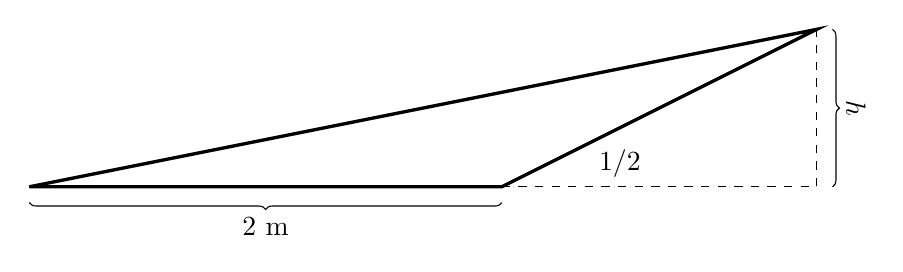
\begin{tikzpicture}
		    \coordinate (B) at (-6,2);
		    \coordinate (C) at (0,2);
		    \coordinate (D) at (4,2);
		    \coordinate (E) at (4,4);
		    \tkzMarkRightAngle(C,D,E)
		    \tkzMarkAngle(D,C,E)
		    \draw[decoration={brace,mirror,raise=.2cm},decorate,thin] (-6,2)--(0,2);
		    \draw[decoration={brace,mirror,raise=.2cm},decorate,thin] (4,2)--(4,4);
%		    \draw[decoration={brace,raise=.2cm},decorate,thin] (0,2)--(4,4);
		    \draw[very thick] (B)--(C)--(E) -- cycle;
		    \draw[dashed] (C)--(D) -- (E);
		    
		    \node at (-3,2-.5) {2 m};
		    \node[rotate=-90] at (4+.5,3) {$h$};
		    \node at (1.5,2.3) {$1/2$};
		  \end{tikzpicture}
		\end{image}
		
		Let us focus on the dotted triangle on the right side		

		\begin{image}[2in]
		  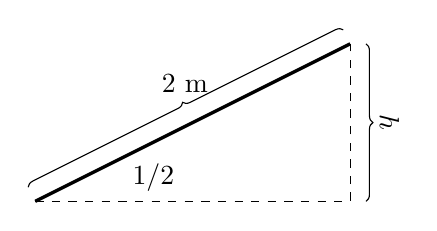
\begin{tikzpicture}
		    \coordinate (C) at (0,2);
		    \coordinate (D) at (4,2);
		    \coordinate (E) at (4,4);
		    \tkzMarkRightAngle(C,D,E)
		    \tkzMarkAngle(D,C,E)
%		    \draw[decoration={brace,mirror,raise=.2cm},decorate,thin] (0,2)--(4,2);
		    \draw[decoration={brace,mirror,raise=.2cm},decorate,thin] (4,2)--(4,4);
		    \draw[decoration={brace,raise=.2cm},decorate,thin] (0,2)--(4,4);
		    \draw[very thick] (E)--(C);
		    \draw[dashed] (C)--(D)--(E);
		    \node at (2-0.1,3+.5) {2 m};
		    \node[rotate=-90] at (4+.5,3) {$h$};
		    \node at (1.5,2.3) {$1/2$};
		  \end{tikzpicture}
		\end{image}
		
		Notice that the height of this right triangle is the same as the height of the obtuse triangle above. Since we know the hypotenuse and base angle of this right triangle, we can find the height (the opposite side) using sine.
		\begin{align*}
			\sin\left( \frac{1}{2} \right) &= \dfrac{h}{2}\\
			2 \sin\left( \frac{1}{2} \right) &= h.
		\end{align*}

		Be careful here! That angle $\frac{1}{2}$ is not in degrees, it's in radians. (You can tell, because there is no ``degrees symbol''.) If you are going to approximate this value, make sure you are using radians.
		
		Now the area of the whole triangle is:
		\begin{align*}
			A 	&= \dfrac{1}{2} b h\\
				&= \dfrac{1}{2} (2)\left( 2 \sin\left( \frac{1}{2} \right)\right)\\
				&= 2 \sin\left( \frac{1}{2} \right).
		\end{align*}

		The exact value of the area is $2 \sin\left( \frac{1}{2} \right) \,m^2$. Using a calculator, this is approximately $0.959\, m^2$. (Remember that $m^2$ is the abbreviation for ``square meters''.)

	\end{explanation}
\end{example}




\begin{example}

	A right triangle is constructed by taking a point $(x,y)$ on the graph of the function $f(x)=\sqrt{x}$, drawing a line vertically downward to
	the $x$-axis, then connecting both of those points to the origin as in the picture below. 	\begin{center}
		  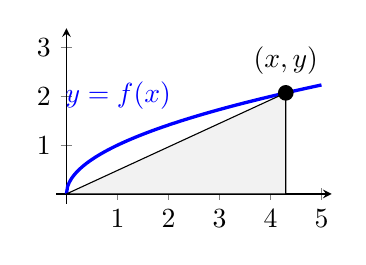
\begin{tikzpicture}
					\begin{axis}[
						xmin=-0.2, xmax=5.2, ymin=-0.2,ymax=3.4,    
						axis lines =middle, 
						every axis y label/.style={at=(current axis.above origin),anchor=south},
						every axis x label/.style={at=(current axis.right of origin),anchor=west},
						xtick={0,...,5}, ytick={0,...,3},
						grid=major, width=2in, height = 1.5in,
						grid style={dashed, gray!0}
						]
						
						\addplot[color=blue, very thick, smooth, samples=200, domain=0:5]{x^(0.5)} node[pos=0.5, above left]{$y=f(x)$};
						\draw[fill=gray!10] (axis cs:0,0) -- (axis cs:4.3, 0) -- (axis cs: 4.3, 2.074) -- cycle;
						\node[label={90:{$(x,y)$}},circle,fill,inner sep=2pt] at (axis cs:4.3,2.074) {};	
%						\draw [thick] (axis cs:0.5,0) arc [radius=0.5,start angle=0,end angle=25.7];		
%						\node[label={0:{$\theta$}},inner sep=2pt] at (axis cs:0.5,0.2) {};	
					\end{axis}

		  \end{tikzpicture}
	\end{center}
	For one particular point $(x,y)$, the acute angle between the hypotenuse of the triangle and the positive $x$-axis is found to measure $\dfrac{\pi}{6}$ radians. Find the coordinates of the point $(x,y)$.

	\begin{explanation}

		Since the hypotenuse of the right triangle runs from the origin, which has coordinates $(0,0)$, to the point $(x,y)$, the horizontal side of the triangle has length $x$ and vertical side has length $y$.
		We know that the value of tangent is given by the ratio of the opposite side length divided by the adjacent side length. Using the given angle of $\dfrac{\pi}{6}$, this means 
		$\tan\left(\dfrac{\pi}{6}\right) = \dfrac{1}{\sqrt{3}} = \dfrac{y}{x}$. That is, $x = y\sqrt{3}$ 
		
		We also know that the point lies on the graph of $f(x) = \sqrt{x}$, which means $y = \sqrt{x}$.
		
		This gives us a nonlinear system of two equations:
		\[ \begin{cases} x = y\sqrt{3} \\ y = \sqrt{x} \end{cases}\]

		Squaring the bottom equation yields $y^2 = x$. When substituting the top equation into the bottom equation, we arrive at:.
		\begin{align*}
			y^2 &= y\sqrt{3}\\
			y^2 - y\sqrt{3} &= 0\\
			y(y - \sqrt{3}) &= 0
		\end{align*}
		so either $y=0$ or $y=\sqrt{3}$.
		
		The value $y=0$ corresponds to the point $(0,0)$ on the graph, which does not yield any angle. This is an extraneous solution, which is discarded.
		
		Substituting the value $y=\sqrt{3}$ into $x = y\sqrt{3}$ gives $x = (\sqrt{3})\sqrt{3} = 3$. The point is $\left( 3, \sqrt{3}\right)$.

	\end{explanation}
\end{example}





\end{document}
